\chapter{AAP}

\hypertarget{introduction-to-ansible-automation-controller}{%
\section{Introduction to Ansible automation
controller}\label{introduction-to-ansible-automation-controller}}

\hypertarget{whats-new-in-ansible-automation-controller-4.0}{%
\subsection{What's New in Ansible automation controller
4.0}\label{whats-new-in-ansible-automation-controller-4.0}}

Ansible Automation Platform 2 is the next evolution in automation from
Red Hat's trusted enterprise technology experts. The Ansible Automation
Platform 2 release includes automation controller 4.0, the improved and
renamed Ansible Tower.

Controller continues to provide a standardized way to define, operate,
and delegate automation across the enterprise. It introduces new
technologies and an enhanced architecture that enables automation teams
to scale and deliver automation rapidly.

\hypertarget{why-was-ansible-tower-renamed-to-automation-controller}{%
\subsubsection{Why was Ansible Tower renamed to automation
controller?}\label{why-was-ansible-tower-renamed-to-automation-controller}}

As Ansible Automation Platform 2 continues to evolve, certain
functionality has been decoupled (and will continue to be decoupled in
future releases) from what was formerly known as Ansible Tower. It made
sense to introduce the naming change that better reflects these
enhancements and the overall position within the Ansible Automation
Platform suite.

\hypertarget{who-is-automation-controller-for}{%
\subsubsection{Who is automation controller
for?}\label{who-is-automation-controller-for}}

All automation team members interact with or rely on automation
controller, either directly or indirectly.

\begin{itemize}
\tightlist
\item
  Automation creators develop Ansible playbooks, roles, and modules.
\item
  Automation architects elevate automation across teams to align with IT
  processes and streamline adoption.
\item
  Automation operators ensure the automation platform and framework are
  operational.
\end{itemize}

These roles are not necessarily dedicated to a person or team. Many
organizations assign multiple roles to people or outsource specific
automation tasks based on their needs.

Automation operators are typically the primary individuals who interact
directly with the automation controller, based on their
responsibilities.

\hypertarget{objective}{%
\subsection{Objective}\label{objective}}

The following exercise will provide an Ansible automation controller
overview including going through features that are provided by the Red
Hat Ansible Automation Platform. This will cover automation controller
fundamentals such as:

\begin{itemize}
\tightlist
\item
  Job Templates
\item
  Projects
\item
  Inventories
\item
  Credentials
\item
  Workflows
\end{itemize}

\hypertarget{guide}{%
\subsection{Guide}\label{guide}}

\hypertarget{why-ansible-automation-controller}{%
\subsubsection{Why Ansible automation
controller?}\label{why-ansible-automation-controller}}

Automation controller is a web-based UI that provides an enterprise
solution for IT automation. It

\begin{itemize}
\tightlist
\item
  has a user-friendly dashboard.
\item
  complements Ansible, adding automation, visual management, and
  monitoring capabilities.
\item
  provides user access control to administrators.
\item
  provides distinct \emph{view} and \emph{edit} perspectives for
  automation controller objects and components.
\item
  graphically manages or synchronizes inventories with a wide variety of
  sources.
\item
  has a RESTful API.
\item
  And much more\ldots{}
\end{itemize}

\hypertarget{your-ansible-automation-controller-lab-environment}{%
\subsubsection{Your Ansible automation controller lab
environment}\label{your-ansible-automation-controller-lab-environment}}

In this lab you work in a pre-configured lab environment. You will have
access to the following hosts:

\begin{longtable}[]{@{}ll@{}}
\toprule\noalign{}
Role & Inventory name \\
\midrule\noalign{}
\endhead
\bottomrule\noalign{}
\endlastfoot
Ansible control host \& automation controller & controller \\
Managed Host 1 & node \\
\end{longtable}

The Ansible automation controller provided in this lab is individually
setup for you. Make sure to access the right machine whenever you work
with it. Automation controller has already been installed and licensed
for you, the web UI will be reachable over HTTP/HTTPS.

\hypertarget{dashboard}{%
\subsubsection{Dashboard}\label{dashboard}}

Let's have a first look at the automation controller: Point your browser
to \texttt{https://10.3.48.100}.

The web UI of automation controller greets you with a dashboard with a
graph showing:

\begin{itemize}
\tightlist
\item
  recent job activity
\item
  the number of managed hosts
\item
  quick pointers to lists of hosts with problems.
\end{itemize}

The dashboard also displays real time data about the execution of tasks
completed in playbooks.

\begin{figure}
\centering
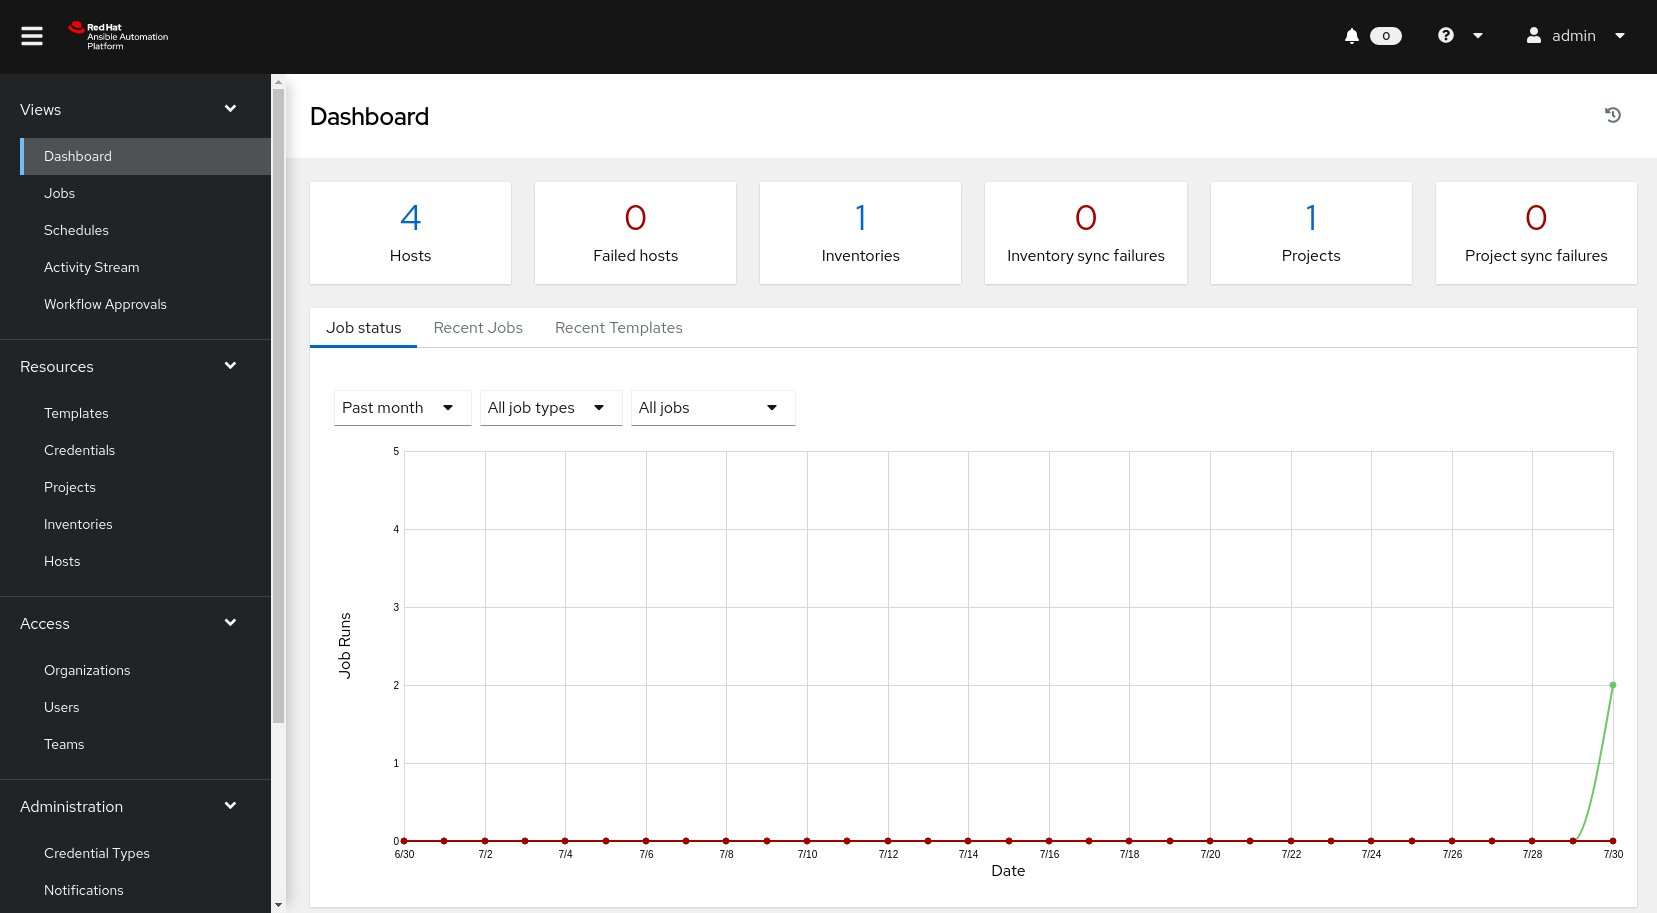
\includegraphics{images/02_controller_dashboard.jpg}
\caption{Ansible automation controller dashboard}
\end{figure}

\hypertarget{concepts}{%
\subsubsection{Concepts}\label{concepts}}

Before we dive further into using Ansible automation controller, you
should get familiar with some concepts and naming conventions.

\hypertarget{projects}{%
\paragraph{Projects}\label{projects}}

Projects are logical collections of Ansible playbooks in Ansible
automation controller. These playbooks either reside on the Ansible
automation controller instance, or in a source code version control
system supported by automation controller.

\hypertarget{inventories}{%
\paragraph{Inventories}\label{inventories}}

An Inventory is a collection of hosts against which jobs may be
launched, the same as an Ansible inventory file. Inventories are divided
into groups and these groups contain the actual hosts. Groups may be
populated manually, by entering host names into automation controller,
from one of Ansible Automation controller's supported cloud providers or
through dynamic inventory scripts.

\hypertarget{credentials}{%
\paragraph{Credentials}\label{credentials}}

Credentials are utilized by automation controller for authentication
when launching Jobs against machines, synchronizing with inventory
sources, and importing project content from a version control system.
Credential configuration can be found in the Settings.

automation controller credentials are imported and stored encrypted in
automation controller, and are not retrievable in plain text on the
command line by any user. You can grant users and teams the ability to
use these credentials, without actually exposing the credential to the
user.

\hypertarget{templates}{%
\paragraph{Templates}\label{templates}}

A job template is a definition and set of parameters for running an
Ansible job. Job templates are useful to execute the same job many
times. Job templates also encourage the reuse of Ansible playbook
content and collaboration between teams. To execute a job, automation
Controller requires that you first create a job template.

\hypertarget{jobs}{%
\paragraph{Jobs}\label{jobs}}

A job is basically an instance of automation controller launching an
Ansible playbook against an inventory of hosts.

\hypertarget{workshop-exercise---inventories-credentials-and-ad-hoc-commands}{%
\section{Workshop Exercise - Inventories, credentials and ad hoc
commands}\label{workshop-exercise---inventories-credentials-and-ad-hoc-commands}}

\hypertarget{objective}{%
\subsection{Objective}\label{objective}}

Explore and understand the lab environment. This exercise will cover

\begin{itemize}
\item
  Locating and understanding:

  \begin{itemize}
  \tightlist
  \item
    Ansible Automation Controller
    \href{https://docs.ansible.com/automation-controller/latest/html/userguide/inventories.html}{\textbf{Inventories}}
  \item
    Ansible Automation Controller
    \href{https://docs.ansible.com/automation-controller/latest/html/userguide/credentials.html}{\textbf{Credentials}}
  \end{itemize}
\item
  Running ad hoc commands via the Ansible Automation Controller web UI
\end{itemize}

\hypertarget{guide}{%
\subsection{Guide}\label{guide}}

\hypertarget{examine-an-inventory}{%
\subsubsection{Examine an Inventory}\label{examine-an-inventory}}

The first thing we need is an inventory of your managed hosts. This is
the equivalent of an inventory file in command-line Ansible. There is a
lot more to it (like dynamic inventories) but let's start with the
basics.

\begin{itemize}
\tightlist
\item
  You should already have the web UI open, if not: Point your browser to
  \texttt{https://10.3.48.100}. The password will be provided by the instructor.
\end{itemize}

There will be one inventory, the \textbf{[USER] Inventory}. Click the
\textbf{[USER] Inventory} then click the \textbf{Hosts} button

The inventory information at
\texttt{\textasciitilde{}/hosts} was pre-loaded into the
Ansible Automation controller Inventory as part of the provisioning
process.

\begin{Shaded}
\begin{Highlighting}[]
\ExtensionTok{$}\NormalTok{ cat \textasciitilde{}/hosts}
\ExtensionTok{[web]}
\ExtensionTok{node}\NormalTok{ ansible\_host=10.3.48.101 ansible\_user=s1}

\ExtensionTok{[control]}
\ExtensionTok{controller}\NormalTok{ ansible\_host=10.3.48.100 ansible\_user=s1}
\end{Highlighting}
\end{Shaded}

\begin{quote}
\textbf{Warning}

In your inventory the IP addresses will be different.
\end{quote}

\hypertarget{examine-machine-credentials}{%
\subsubsection{Examine Machine
Credentials}\label{examine-machine-credentials}}

Now we will examine the credentials to access our managed hosts from
Automation controller. As part of the provisioning process for this
Ansible Workshop the \textbf{[USER] Credential} has already been
setup.

In the \textbf{Resources} menu choose \textbf{Credentials}. Now click on
the \textbf{[USER] Credential}.

Note the following information:
\begin{itemize}
        \tightlist
    \item \textbf{Credential Type}: Machine- Machine credentials define ssh and user-level privilege
escalation access for playbooks. They are used when submitting jobs to
run playbooks on a remote host.
\item \textbf{Username}: matches our command-line Ansible inventory username for
the other Linux nodes
\item \textbf{SSH Private Key}: Encrypted - take note that you can't actually examine the SSH private
key once someone hands it over to Ansible Automation controller
\end{itemize}

\hypertarget{run-ad-hoc-commands}{%
\subsubsection{Run Ad Hoc commands}\label{run-ad-hoc-commands}}

It is possible to run run ad hoc commands from Ansible Automation
controller as well.

\begin{itemize}
\item
  In the webUI go to \textbf{Resources → Inventories → [USER]
  Inventory}
\item
  Click the \textbf{Hosts} tab to change into the hosts view and select
  the \texttt{node} host by ticking the box to the left of the host entry.
\item
  Click \textbf{Run Command} button. In the next screen you have to
  specify the ad hoc command.
\end{itemize}

Within the \textbf{Details} window, select \textbf{Module} \texttt{ping}
and click \textbf{Next}.

Within the \textbf{Execution Environment} window, select \textbf{Default
execution environment} and click \textbf{Next}.

Within the \textbf{Machine Credential} window, select \textbf{[USER]
Credentials} and click \textbf{Launch}.

\begin{quote}
\textbf{Tip}

The output of the results is displayed once the command has completed.
\end{quote}

The simple \textbf{ping} module doesn't need options. For other modules
you need to supply the command to run as an argument. Try the
\textbf{command} module to find the userid of the executing user using
an ad hoc command.

\begin{itemize}
\item
    In the web UI go to \textbf{Resources → Inventories → [USER]
  Inventory}
\item
  Click the \textbf{Hosts} tab to change into the hosts view and select
  the \texttt{node} host by ticking the box to the left of the host entry.
\item
  Click \textbf{Run Command} button. In the next screen you have to
  specify the ad hoc command.
\end{itemize}

Within the \textbf{Details} window, select \textbf{Module}
\texttt{command}, in \textbf{Arguments} type \texttt{id} and click
\textbf{Next}.

Within the \textbf{Execution Environment} window, select \textbf{Default
execution environment} and click \textbf{Next}.

Within the \textbf{Machine Credential} window, select \textbf{[USER]
Credentials} and click \textbf{Launch}.

\begin{quote}
\textbf{Tip}

After choosing the module to run, Ansible Automation Controller will
provide a link to the docs page for the module when clicking the
question mark next to ``Arguments''. This is handy, give it a try.
\end{quote}

How about trying to get some secret information from the system? Try to
print out \emph{/etc/shadow}.

\begin{itemize}
\item
    In the web UI go to \textbf{Resources → Inventories → [USER]
  Inventory}
\item
  Click the \textbf{Hosts} tab to change into the hosts view and select
  the \texttt{node} host by ticking the box to the left of the host entry.
\item
  Click \textbf{Run Command} button. In the next screen you have to
  specify the ad hoc command.
\end{itemize}

Within the \textbf{Details} window, select \textbf{Module}
\texttt{command}, in \textbf{Arguments} type \texttt{cat\ /etc/shadow}
and click \textbf{Next}.

Within the \textbf{Execution Environment} window, select \textbf{Default
execution environment} and click \textbf{Next}.

Within the \textbf{Machine Credential} window, select \textbf{[USER]
Credentials} and click \textbf{Launch}.

\begin{quote}
\textbf{Warning}

\textbf{Expect an error!}
\end{quote}

Oops, the last one didn't went well, all red.

Re-run the last ad hoc command but this time check the checkbox labeled
\textbf{Enable privilege escalation}.

As you see, this time it worked. For tasks that have to run as
\texttt{root} you need to escalate the privileges. This is the same as
the \textbf{become: True} used in your Ansible Playbooks.

\hypertarget{challenge-lab-ad-hoc-commands}{%
\subsubsection{Challenge Lab: Ad Hoc
Commands}\label{challenge-lab-ad-hoc-commands}}

Okay, a small challenge: Run an ad hoc to make sure the package ``tmux''
is installed on all hosts. If unsure, consult the documentation either
via the web UI as shown above or by running
\texttt{{[}ansible@controller\ \textasciitilde{}{]}\$\ ansible-doc\ yum}
on your Automation controller control host.

\begin{quote}
\textbf{Warning}

\textbf{Solution below!}
\end{quote}

\begin{itemize}
\item
    In the web UI go to \textbf{Resources → Inventories → [USER]
  Inventory}
\item
  Click the \textbf{Hosts} tab to change into the hosts view and select
  the \texttt{node} host by ticking the box to the left of the host entry.
\item
  Click \textbf{Run Command} button. In the next screen you have to
  specify the ad hoc command.
\end{itemize}

Within the \textbf{Details} window, select \textbf{Module} \texttt{yum},
in \textbf{Arguments} type \texttt{name=tmux}, check \textbf{Enable
privilege escalation} and click \textbf{Next}.

Within the \textbf{Execution Environment} window, select \textbf{Default
execution environment} and click \textbf{Next}.

Within the \textbf{Machine Credential} window, select \textbf{[USER]
Credentials} and click \textbf{Launch}.

\begin{quote}
\textbf{Tip}

Notice how the package was instaled via the ``CHANGED'' output. If you
run the ad hoc command a second time, the output will mention
``SUCCESS'' and inform you via the message parameter that there is
nothing to do.
\end{quote}

\hypertarget{workshop-exercise---projects-job-templates}{%
\section{Workshop Exercise - Projects \& Job
Templates}\label{workshop-exercise---projects-job-templates}}

\hypertarget{objective}{%
\subsection{Objective}\label{objective}}

An Ansible automation controller \textbf{Project} is a logical
collection of Ansible playbooks. You can manage your playbooks by
placing them into a source code management (SCM) system supported by
automation controller such as Git or Subversion.

This exercise covers:

\begin{itemize}
\tightlist
\item
  Understanding and using an Ansible automation controller Project
\item
  Using Ansible playbooks kept in a Git repository.
\item
  Creating and using an Ansible Job Template
\end{itemize}

\hypertarget{guide}{%
\subsection{Guide}\label{guide}}

\hypertarget{setup-git-repository}{%
\subsubsection{Setup Git Repository}\label{setup-git-repository}}

For this demonstration we will use playbooks stored in a Git repository:

\url{https://github.com/ansible/workshop-examples}

A playbook to install the Apache web server has already been committed
to the directory \textbf{rhel/apache}, \texttt{apache\_install.yml}:

\begin{Shaded}
\begin{Highlighting}[]
\PreprocessorTok{{-}{-}{-}}
\KeywordTok{{-}}\AttributeTok{ }\FunctionTok{name}\KeywordTok{:}\AttributeTok{ Apache server installed}
\AttributeTok{  }\FunctionTok{hosts}\KeywordTok{:}\AttributeTok{ web}

\AttributeTok{  }\FunctionTok{tasks}\KeywordTok{:}
\AttributeTok{  }\KeywordTok{{-}}\AttributeTok{ }\FunctionTok{name}\KeywordTok{:}\AttributeTok{ latest Apache version installed}
\AttributeTok{    }\FunctionTok{ansible.builtin.yum}\KeywordTok{:}
\AttributeTok{      }\FunctionTok{name}\KeywordTok{:}\AttributeTok{ httpd}
\AttributeTok{      }\FunctionTok{state}\KeywordTok{:}\AttributeTok{ latest}

\AttributeTok{  }\KeywordTok{{-}}\AttributeTok{ }\FunctionTok{name}\KeywordTok{:}\AttributeTok{ latest firewalld version installed}
\AttributeTok{    }\FunctionTok{ansible.builtin.yum}\KeywordTok{:}
\AttributeTok{      }\FunctionTok{name}\KeywordTok{:}\AttributeTok{ firewalld}
\AttributeTok{      }\FunctionTok{state}\KeywordTok{:}\AttributeTok{ latest}

\AttributeTok{  }\KeywordTok{{-}}\AttributeTok{ }\FunctionTok{name}\KeywordTok{:}\AttributeTok{ firewalld enabled and running}
\AttributeTok{    }\FunctionTok{ansible.builtin.service}\KeywordTok{:}
\AttributeTok{      }\FunctionTok{name}\KeywordTok{:}\AttributeTok{ firewalld}
\AttributeTok{      }\FunctionTok{enabled}\KeywordTok{:}\AttributeTok{ }\CharTok{true}
\AttributeTok{      }\FunctionTok{state}\KeywordTok{:}\AttributeTok{ started}

\AttributeTok{  }\KeywordTok{{-}}\AttributeTok{ }\FunctionTok{name}\KeywordTok{:}\AttributeTok{ firewalld permits http service}
\AttributeTok{    }\FunctionTok{ansible.builtin.firewalld}\KeywordTok{:}
\AttributeTok{      }\FunctionTok{service}\KeywordTok{:}\AttributeTok{ http}
\AttributeTok{      }\FunctionTok{permanent}\KeywordTok{:}\AttributeTok{ }\CharTok{true}
\AttributeTok{      }\FunctionTok{state}\KeywordTok{:}\AttributeTok{ enabled}
\AttributeTok{      }\FunctionTok{immediate}\KeywordTok{:}\AttributeTok{ }\CharTok{yes}

\AttributeTok{  }\KeywordTok{{-}}\AttributeTok{ }\FunctionTok{name}\KeywordTok{:}\AttributeTok{ Apache enabled and running}
\AttributeTok{    }\FunctionTok{ansible.builtin.service}\KeywordTok{:}
\AttributeTok{      }\FunctionTok{name}\KeywordTok{:}\AttributeTok{ httpd}
\AttributeTok{      }\FunctionTok{enabled}\KeywordTok{:}\AttributeTok{ }\CharTok{true}
\AttributeTok{      }\FunctionTok{state}\KeywordTok{:}\AttributeTok{ started}
\end{Highlighting}
\end{Shaded}

\begin{quote}
\textbf{Tip}

Note the difference to other playbooks you might have written! Most
importantly there is no \texttt{become} and \texttt{hosts} is set to
\texttt{all}.
\end{quote}

To configure and use this repository as a \textbf{Source Control
Management (SCM)} system in automation controller you have to create a
\textbf{Project} that uses the repository

\hypertarget{create-the-project}{%
\subsubsection{Create the Project}\label{create-the-project}}

\begin{itemize}
\tightlist
\item
  Go to \textbf{Resources → Projects} click the \textbf{Add} button.
  Fill in the form:

        \begin{itemize}
            \item \textbf{Name}: Workshop Project
            \item \textbf{Organization}: [USER]
            \item \textbf{Default Execution Environment}: Default execution environment
            \item \textbf{Source Control Credential Type}: Git
            \item Enter the URL into the \textbf{Project configuration}
            \item \textbf{Source Control URL}: https://github.com/ansible/workshop-examples.git
            \item \textbf{Options}: Select Clean, Delete, Update Revision on Launch to request a fresh copy
of the repository and to update the repository when launching a job.

\end{itemize}
\item
  Click \textbf{SAVE}
\end{itemize}

The new project will be synced automatically after creation. But you can
also do this manually: Sync the Project again with the Git repository by
going to the \textbf{Projects} view and clicking the circular arrow
\textbf{Sync Project} icon to the right of the Project.

After starting the sync job, go to the \textbf{Jobs} view: there is a
new job for the update of the Git repository.

\hypertarget{create-a-job-template-and-run-a-job}{%
\subsubsection{Create a Job Template and Run a
Job}\label{create-a-job-template-and-run-a-job}}

A job template is a definition and set of parameters for running an
Ansible job. Job templates are useful to execute the same job many
times. So before running an Ansible \textbf{Job} from automation
controller you must create a \textbf{Job Template} that pulls together:

\begin{itemize}
\item
  \textbf{Inventory}: On what hosts should the job run?
\item
  \textbf{Credentials} What credentials are needed to log into the
  hosts?
\item
  \textbf{Project}: Where is the playbook?
\item
  \textbf{What} playbook to use?
\end{itemize}

Okay, let's just do that: Go to the \textbf{Resources -\textgreater{}
Templates} view, click the \textbf{Add} button and choose \textbf{Add
job template}.

\begin{quote}
\textbf{Tip}

Remember that you can often click on magnfying glasses to get an
overview of options to pick to fill in fields.
\end{quote}
\begin{itemize}
\tightlist
    \item \textbf{Name}: Install Apache
    \item \textbf{Job Type}: Run
    \item \textbf{Inventory}: [USER] Inventory
    \item \textbf{Project}: Workshop Project
    \item \textbf{Execution Environment}: Default execution environment
    \item \textbf{Playbook}: rhel/apache/apache\_install.yml
    \item \textbf{Credentials}: [USER] Credential
    \item \textbf{Limit}: web
    \item tasks need to run as root so check \textbf{Privilege Escalation}
\end{itemize}

\begin{itemize}
\tightlist
\item
  Click \textbf{Save}
\end{itemize}

You can start the job by directly clicking the blue \textbf{Launch}
button, or by clicking on the rocket in the Job Templates overview.
After launching the Job Template, you are automatically brought to the
job overview where you can follow the playbook execution in real time:

Job Details 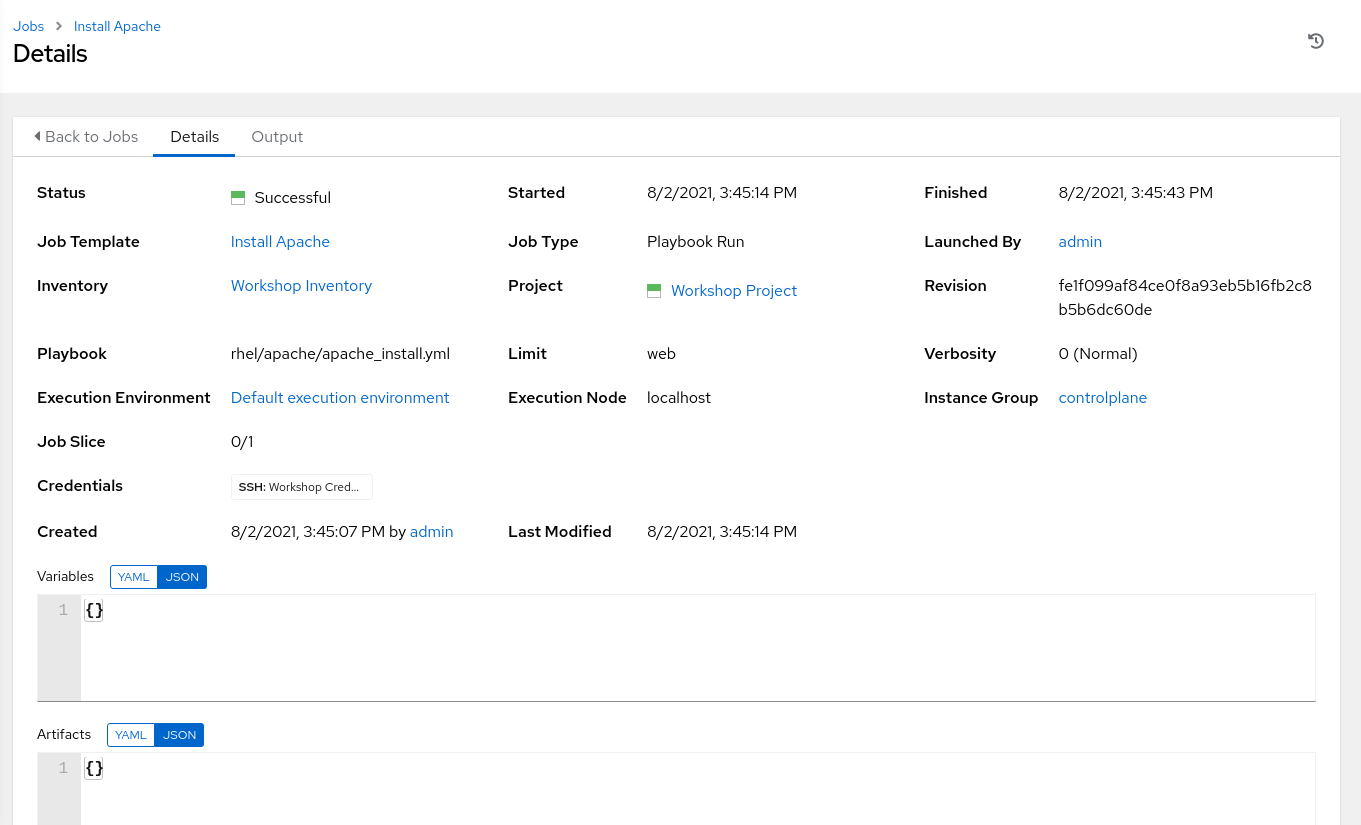
\includegraphics{images/02_job_details.png}

Job Run 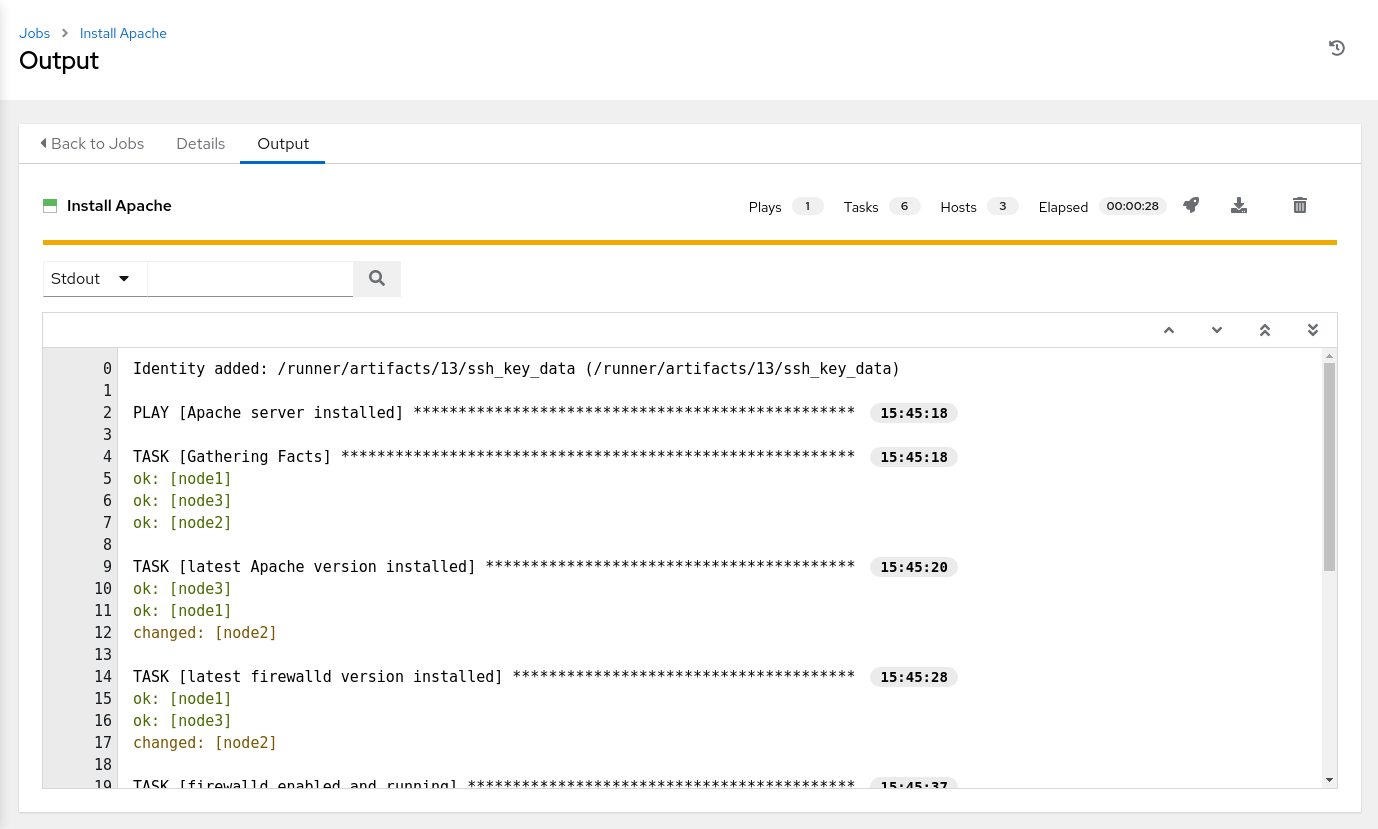
\includegraphics{images/02_job_run.png}

Since this might take some time, have a closer look at all the details
provided:

\begin{itemize}
\item
  All details of the job template like inventory, project, credentials
  and playbook are shown.
\item
  Additionally, the actual revision of the playbook is recorded here -
  this makes it easier to analyse job runs later on.
\item
  Also the time of execution with start and end time is recorded, giving
  you an idea of how long a job execution actually was.
\item
  Selecting \textbf{Output} shows the output of the running playbook.
  Click on a node underneath a task and see that detailed information
  are provided for each task of each node.
\end{itemize}

After the Job has finished go to the main \textbf{Jobs} view: All jobs
are listed here, you should see directly before the Playbook run an
Source Control Update was started. This is the Git update we configured
for the \textbf{Project} on launch!

\hypertarget{challenge-lab-check-the-result}{%
\subsubsection{Challenge Lab: Check the
Result}\label{challenge-lab-check-the-result}}

Time for a little challenge:

\begin{itemize}
\tightlist
\item
  Use an ad hoc command on both hosts to make sure Apache has been
  installed and is running.
\end{itemize}

You have already been through all the steps needed, so try this for
yourself.

\begin{quote}
\textbf{Tip}

What about \texttt{systemctl\ status\ httpd}?
\end{quote}

\begin{quote}
\textbf{Warning}

\textbf{Solution Below}
\end{quote}

\begin{itemize}
\item
  Go to \textbf{Resources → Inventories} → \textbf{[USER] Inventory}
\item
  In the \textbf{Hosts} view select \texttt{node} and click \textbf{Run Command}
\end{itemize}

Within the \textbf{Details} window, select \textbf{Module}
\texttt{command}, in \textbf{Arguments} type
\texttt{systemctl\ status\ httpd} and click \textbf{Next}.

Within the \textbf{Execution Environment} window, select \textbf{Default
execution environment} and click \textbf{Next}.

Within the \textbf{Machine Credential} window, select \textbf{[USER]
Credential} and click \textbf{Launch}.

\begin{quote}
\textbf{Tip}

The output of the results is displayed once the command has completed.
\end{quote}

\hypertarget{workshop-exercise---role-based-access-control}{%
\section{Workshop Exercise - Role-based access
control}\label{workshop-exercise---role-based-access-control}}

\hypertarget{objective}{%
\subsection{Objective}\label{objective}}

You have already learned how Ansible automation controller separates
credentials from users. Another advantage of Ansible automation
controller is the user and group rights management. This exercise
demonstrates Role Based Access Control (RBAC)

\hypertarget{guide}{%
\subsection{Guide}\label{guide}}

\hypertarget{ansible-automation-controller-users}{%
\subsubsection{Ansible automation controller
users}\label{ansible-automation-controller-users}}

There are three types of automation controller users:

\begin{itemize}
\item
  \textbf{Normal User}: Have read and write access limited to the
  inventory and projects for which that user has been granted the
  appropriate roles and privileges.
\item
  \textbf{System Auditor}: Auditors implicitly inherit the read-only
  capability for all objects within the automation controller
  environment.
\item
  \textbf{System Administrator}: Has admin, read, and write privileges
  over the entire automation controller installation.
\end{itemize}

Let's create a user:

\begin{itemize}
\item
  In the automation controller menu under \textbf{Access} click
  \textbf{Users}
\item
  Click the \textbf{Add} button
\item
  Fill in the values for the new user:

        \begin{itemize}
            \item \textbf{Username}: [USER]-wweb
            \item \textbf{Password}: ansible
            \item \textbf{Confirm Password}: ansible
            \item \textbf{Organization}: [USER]
            \item \textbf{User Type}: Normal User
        \end{itemize}

\item
  Click \textbf{Save}
\end{itemize}

\hypertarget{ansible-automation-controller-teams}{%
\subsubsection{Ansible automation controller
teams}\label{ansible-automation-controller-teams}}

A Team is a subdivision of an organization with associated users,
projects, credentials, and permissions. Teams provide a means to
implement role-based access control schemes and delegate
responsibilities across organizations. For instance, permissions may be
granted to a whole Team rather than each user on the Team.

Create a Team:

\begin{itemize}
\item
  In the menu go to \textbf{Access → Teams}
\item
  Click the \textbf{Add} button and create a team named
  \texttt{[USER] Web\ Content} within the \texttt{[USER]} Organization.
\item
  Click \textbf{Save}
\end{itemize}

Add a user to the team:

\begin{itemize}
\item
  Click on the team \texttt{[USER] Web\ Content} and click the \textbf{Access}
  tab and click \textbf{Add}.
\item
  Within the \textbf{Select a Resource Type} window, click on the
  \textbf{Users} resource type and click \textbf{Next}.
\item
  Within the \textbf{Select Items from List}, select the checkbox next
  to the \texttt{[USER]-wweb} user and click \textbf{Next}.
\item
  Within the \textbf{Select Roles to Apply}, select \textbf{Member} as
  the role to apply to the \texttt{[USER]-wweb} user.
\end{itemize}

Click \textbf{Save}.

Permissions allow to read, modify, and administer projects, inventories,
and other automation controller elements. Permissions can be set for
different resources.

\hypertarget{granting-permissions}{%
\subsubsection{Granting permissions}\label{granting-permissions}}

To allow users or teams to actually do something, you have to set
permissions. The user \textbf{[USER]-wweb} should only be allowed to modify
content of the assigned webservers.

Add the permission to use the \texttt{Create\ index.html} template:

\begin{itemize}
\item
  Within \textbf{Resources} -\textgreater{} \textbf{Templates}, select
  \texttt{Create\ index.html}.
\item
  Select \textbf{Access} tab from the menu and click \textbf{Add}.
\item
  Within the \textbf{Select a Resource Type} window, click on the
  \textbf{Users} resource type and click \textbf{Next}.
\item
  Within the \textbf{Select Items from List}, select the checkbox next
  to the \texttt{[USER]-wweb} user and click \textbf{Next}.
\item
  Within the \textbf{Select Roles to Apply}, select \textbf{Read} and
  \textbf{Execute} as the roles to apply to the \texttt{[USER]-wweb} user.
\item
  Click \textbf{Save}
\end{itemize}

\hypertarget{test-permissions}{%
\subsubsection{Test permissions}\label{test-permissions}}

Now log out of automation controller's web UI and in again as the
\textbf{[USER]-wweb} user.

\begin{itemize}
\item
  Go to the \textbf{Templates} view, you should notice for wweb only the
  \texttt{Create\ \ \ index.html} template is listed. He is allowed to
  view and launch, but not to edit the Template (no Edit button
  available).
\item
  Run the Job Template by clicking the rocket icon. Enter the values for
  the survey questions and launch the job.
\item
  In the following \textbf{Jobs} view have a good look around, note that
  there where changes to the host (as expected).
\end{itemize}

Check the result: execute \texttt{curl} again on the control host to
pull the content of the webserver on \texttt{node}:

\begin{Shaded}
\begin{Highlighting}[]
\CommentTok{\#\textgreater{} curl http://10.3.48.[100+PARTICIPANT\_ID]}
\end{Highlighting}
\end{Shaded}

Just recall what you have just done: You enabled a restricted user to
run an Ansible playbook

\begin{itemize}
\item
  Without having access to the credentials
\item
  Without being able to change the playbook itself
\item
  But with the ability to change variables you predefined!
\end{itemize}

Effectively you provided the power to execute automation to another user
without handing out your credentials or giving the user the ability to
change the automation code. And yet, at the same time the user can still
modify things based on the surveys you created.

This capability is one of the main strengths of Ansible automation
controller!
